%===============================================================================
% $Id: ifacconf.tex 19 2011-10-27 09:32:13Z jpuente $  
% Template for IFAC meeting papers
% Copyright (c) 2007-2008 International Federation of Automatic Control
%===============================================================================
\documentclass{ifacconf}

\usepackage{graphicx}      % include this line if your document contains figures
\usepackage{amsfonts}
\usepackage{amsmath}
\usepackage{natbib}        % required for bibliography
\usepackage{multirow}
\usepackage[dvipsnames]{xcolor}

%===============================================================================
\begin{document}
\begin{frontmatter}

\title{Learning Energy Efficient Jumping Strategies for Flexible-Legged Systems} 
% Title, preferably not more than 10 words.

\author[First]{Andrew Albright} 
\author[Second]{Joshua Vaughan} 

\address[First]{University of Louisiana at Lafayette, 
   Lafayette, LA 70503 USA (andrew.albright1@louisiana.edu)}
\address[Second]{University of Louisiana at Lafayette, 
   Lafayette, LA 70503 USA (joshua.vaughan@louisiana.edu)}

\begin{abstract}                % Abstract of not more than 250 words.
   Legged locomotive systems have many advantages over their wheeled counterparts, such as their ability to navigate rough terrain. There are many techniques to overcome obstacles, one of which is jumping. Still, there are disadvantages to overcome when using legged systems, such as their lack of energy efficiency. To combat this lack of efficiency, flexible links can be used to conserve energy that would otherwise be wasted during locomotion. Furthermore, control methods that improve a jumping system's ability to jump high and its ability to conserve power can be utilized. In this paper, reinforcement learning (RL) was used to create controllers for a flexible-legged jumping system that maximize jump height while minimizing power usage.
\end{abstract}

\begin{keyword}
Power Efficient, Reinforcement Learning, Flexible Robots, Legged Locomotion, Jumping
\end{keyword}

\end{frontmatter}
%===============================================================================


\section{Introduction}
   Legged locomotive robots have many advantages over their wheeled counterparts, a major one being their ability to more easily navigate harshly uneven terrain (\cite{Park2017, Blackman2018, Seok2015}). However, there are disadvantages as well, one of which is power consumption. There are several factors that contribute to this disadvantage. For example, multi-legged systems require several motors per leg, and often actuating all motors is required to locomote. In contrast a wheeled system may need only a single motor to turn a set of wheels to accomplish the same task. Another factor, one that is particularly prevalent when navigating uneven terrain, is the challenge of defining how a walking robot places its feet in such a way that reduces wasted footfall energy while maintaining stability.

   In an effort to alleviate the power consumption issues seen when using legged systems, research has been conducted which replaces rigid aspects of said systems with flexible ones. It has been shown that this not only leads to higher performance but also higher efficiency (\cite{Sugiyama2004, Galloway2011, Hurst2008, Seok2015}).

   While the introduction of flexible components solves some challenges related to performance measures like power consumption, it raises other challenges. Modeling the systems becomes more difficult because the models become highly nonlinear. Different approaches have been taken to mitigate these issues, a popular and successful example being the use of series elastic actuators instead of flexible links (\cite{Pratt1995, Iida2005, Ahmadi1997}). Other solutions seek to create control methods which are suited to non-rigid systems. One of those control methods is reinforcement learning (RL), which creates controllers based on learned control strategies that are developed through interactions with an environment. These RL controllers are typically called control agents or just agents.
   
   In this work, reinforcement learning is used to develop control strategies for a simplified jumping robot. The RL agent is trained to maximize jump height while conserving power. The next section will look at some related work in the fields of RL, flexible systems, and power conservative-control strategies. In Section 3, a description of the environment used for training and evaluating the RL agents will be provided. A short description of the RL algorithm used for this work is presented in Section 4. Then, in Section 5, a breakdown of the reward functions used to train the agents is provided. The experiments performed are discussed in Section 6, and evaluations are provided in Section 7. Finally, in Section 8, conclusive remarks will be made. 


\section{Previous Work}
   \subsection{Reinforcement Learning for Legged Locomotion}  
      Research has shown that using RL for defining control strategies for legged systems is a viable path for both simple and complex legged locomotive systems (\cite{Reda2020c}). Using a model-based method has been shown to reduce the number of environment interactions during controller training by an order of magnitude when compared to model-free methods (\cite{Yang2019}). However, model-based methods expose other challenges. Learning a model often requires many interactions, and the inevitably limited environment that is learned leads to limited exploration during controller training. As such, model-free methods are often of interest as they can be deployed directly on hardware to learn based on interactions with the environment. Alternatively, they can be trained initially in simulation on a non-perfect model, then moved to hardware to finish training. An example of success seen in model-free methods is the work which uses RL to train multiple agents to locomote while navigating uneven terrain (\cite{Peng2016}). Still, model-free methods have a host of difficulties to overcome. One in particular is the unreliability seen when finding control strategies, which in many cases is related to training environment definitions (\cite{Reda2020c}).
      
   \subsection{Reinforcement Learning for Flexible Systems} 
      As discussed, flexible systems do have some advantages over their rigid counterparts, particularly ones which are used for locomotion tasks. Typically, for model-based RL methods used for flexible systems, learning a controller is necessary as the model of the system is usually difficult to create (\cite{Thuruthelb}). To avoid the difficulties associated with learning a model of an environment, model-free methods have been deployed for flexible systems and show the potential of controllers that do not require a model of the system (\cite{Dwiel2019d}). Additionally, comparing RL control strategies to PD contrast strategies, it has been shown that RL is practically applicable for controlling flexible systems (\cite{He2020f}). Furthermore, RL control can be used for partial control of flexible systems, an example being the use of an RL controller to limit vibration while a separate controller is used to determine general pose (\cite{Cui2019e}).  

   \subsection{Improving Performance with Flexible Robots} 
      Using flexible components within robotic systems has shown great potential for conserving power. Of the different approaches taken, a popular and proven technique is the use of series-elastic actuators to increase energy efficiency (\cite{Pratt1995, Ahmadi1997}). Similarly, the use of series elastic actuation to capture otherwise wasted foot fall energy has been shown as an effective way of increasing efficiency (\cite{Seok2013, Seok2015}). Flexible joints are not the only way to increase efficiency though; a technique which seeks to emulate the tendons seen in nature has produced similar results (\cite{Folkertsma2012}). Additionally, performance comparisons of flexible and rigid system designs have been made, and the data shows that adding flexible components can increase certain performance measures. For example, the use of a flexible spine in a 2D running robot enabled drastic increases in forward velocity performance (\cite{Kani2013}). 
   
   \subsection{Control for Power Efficiency}
      Rather than relying solely on the mechanical design of a system to increase efficiency, control techniques can be employed to increase power conservation. An example being the use of model predictive control methods that lead to more efficient locomotion strategies (\cite{Harper2019}). In contrast to studying traditional methods of control to accomplish energy efficient strategies, little work has been done to evaluate the potential of using RL control strategies to directly effect power efficiency.
      
      
\section{Pogo-stick Environment}
   A simplified model of a flexible-legged jumping system is the pogo-stick model shown in Fig.~\ref{fig:JumpingModel}.  This model can be used as a base representation for many different jumping animals (\cite{Blickhan1993a}). As such, this model was used as an environment to evaluate the viability of using RL to define control strategies for flexible systems.
   
   \begin{figure}[tb]
         \begin{center}
            \includegraphics[width=2.5cm]{figures/pogo_system.pdf}    % The printed column width is 8.4 cm.
            \caption{Pogo-stick Model for a Simplified Flexible-Legged Jumping System} 
            \label{fig:JumpingModel}
         \end{center}
         \vspace{0.25cm}
      \end{figure}
      
      \begin{table}[tb]
         \begin{center}
         \caption{Training and Evaluation Parameters}\label{tab:JumpingModelParameters}
            \begin{tabular}{cccc}
               \hline
               \hline 
               Model Parameter & Value \\ 
               \hline 
               Mass of Leg, $m_l$ & 0.175 kg \\ 
               Mass of Actuator, $m_a$ & 1.003 kg \\ 
               Natural Frequency, $\omega_n$ & 11.13 Hz \\ 
               Spring Constant, $k$ & 200000 $\mbox{N/m}$ \\ 
               \hline
               Actuator Stroke, $(x_a)_{\mbox{max}}$ & 25 mm \\
               Actuator Velocity, $(\dot{x}_a)_{\mbox{max}}$ & 2.0 $\mbox{m/s}$ \\
               Actuator Acceleration, $(\ddot{x}_a)_{\mbox{max}}$ & 10 $\mbox{m/s}$ \\ \hline \hline
            \end{tabular}
         \end{center}
         \vspace{4mm}
      \end{table}

      Launching the pogo-stick into the air requires the agent to to accelerate the mass, $m_a$, along the rod, $m_l$. The masses of the actuator and leg are represented by $m_a$ and $m_l$, respectively. A nonlinear spring with constant $k$ is used as a flexible component. A damper (not shown in Fig.~\ref{fig:JumpingModel}) is parallel to the spring and is represented by the variable $c$. The vertical position relative to the ground is represented by $x$, and the position which the actuator moves along the rod is represented by $x_a$. The system is constrained to move vertically so that the agent does not learn to keep the system balanced. The values of these system parameters used in the work presented in this paper are detailed in Table~\ref{tab:JumpingModelParameters}.

      The equations of motion for the system are:

      \begin{equation}
         \ddot{x} = \alpha \left(\frac{k}{m_t}x^3+\frac{c}{m_t}\dot{x}\right)-\frac{m_a}{m_t}\,\ddot{x}_a-g
      \end{equation}

      where $x$ and $\dot{x}$ are position and velocity of the rod, respectively, $\ddot{x}_a$ is the acceleration of the actuator as well as the control input, and $m_t$ is the mass of the complete system. Ground contact determines the value of $\alpha$, so that the spring and damper do not supply force while the leg is airborne:

      \begin{equation}
         \alpha =
         \left\{\begin{matrix}
            -1, & x \leq 0\\ 
            0, & \mbox{otherwise}
            \end{matrix}\right.
      \end{equation}
      

\section{Reinforcement Learning}
   % Learning the environment is defined by a Markov Decision Process (MDP) where there exists a set of states $\mathcal{S}$, a set of actions $\mathcal{A}$, a transition probability function $p: \mathcal{S} \times \mathcal{A} \rightarrow \mathcal{P(S)}$, a reward function $R: \mathcal{S} \times \mathcal{S} \times \mathcal{A} \rightarrow \mathbb{R}$, and a future discounting factor $\gamma \in [0,1]$. Iteratively stepping through the MDP will generate a policy $\pi_{\phi}: \mathcal{S} \rightarrow \mathcal{A}$ where the parameters $\phi$ are defined so that all $s_0 \in \mathcal{S}$ have a defined maximum $J(\phi)=\mathbb{E} \left [ \sum_{t=0}^{\infty} \gamma^t R(s_{t+1}, s_t, a_t) \right ]$, being the expected reward.

   For the experiments in this work, a traditional reinforcement learning environment and setup was utilized. The algorithm used was the Stable Baselines implementation of Twin Delayed Deep Deterministic Policy Gradient (TD3) (\cite{Fujimoto2018d}). This is a slightly more advanced version of the popular Deep Deterministic Policy Gradient (DDPG) algorithm which has been used in a host of different applications (\cite{Lillicrap2016h, Bhagat2019e, Dwiel2019d, Ha2018a, Cui2019e}).
   
   TD3 is an actor-critic, off-policy RL algorithm wherein the actor is represented by a policy $\pi_{\phi}$ taking actions $\mathcal{A}$. The critic is represented by the estimated expected return of taking action $\mathcal{A}$ in state $\mathcal{S}$ and following the policy $\pi$ from then after. The critic is a neural network that is updated according to the temporal difference error found between a set of twin target networks. These target networks are updated to follow the critic network every defined $n$ updates of the critic network. The hyperameters used for the experiments in this work can be found in Table~\ref{tab:AlgorithmHyperameters}.

   \begin{table}[tb]
      \begin{center}
      \caption{TD3 Algorithm Hyperparameters}\label{tab:AlgorithmHyperameters}
         \begin{tabular}{cccc}
            \hline
            \hline 
            Algorithm Hyperparameter & Value \\ 
            \hline 
            Learning Rate, $\alpha$ & 0.001 \\ 
            Buffer Size, $\mathcal{D}$ & 500k \\ 
            Learning Starts & 10k \\ 
            Batch Size & 100 \\
            Polyak Update, $\tau$ & 0.005 \\
            Discount Factor, $\gamma$ & 0.99 \\ 
            Update Frequency & 1/episode \\
            Gradient Steps & $\equiv$ previous episode steps \\
            Policy Delay & 2 \\
            Target Policy Noise & 0.2 \\
            Target Noise Clip & 0.5 \\
            Seed & See Table~\ref{tab:trainingSchedule} \\
            \hline \hline
         \end{tabular}
      \end{center}
   \end{table}


\section{Reward Functions}

   \subsection{Rewarding the Agent for Jumping High}
      To accomplish the task of maximizing jump height, a reward function which represents the height of the pogo-stick above the ground at any given time step was used. The signal returned to the agent was normalized with a predefined maximum height, so that if the pogo-stick was at or above that maximum, the agent received maximum reward. This reward function is:

      \begin{equation} \label{eq:rewardHeight}
         r = \frac{x_t - x_{min}}{x_{max} - x_{min}}
      \end{equation}

      where $x_t$ is the height at the current time step, $x_{min}$ is the minimum height of the system, and $x_{max}$ is the maximum height of the system, which is set based on expectations gathered from experimental data. In this work, it was 0.9~meters.

   \subsection{Rewarding the Agent for Jumping Efficiently}
      The second reward function used is one that seeks to balance jumping height with power consumption. To do this, the reward signal returned at each time step is the ratio of the current height to the power used from time zero to the current time step. The power used at a given time step is defined by:
      
      \begin{equation} \label{eq:powerWRTTime}
         p_t = m_a\,\ddot{x}_{a_{t}}\,\dot{x}_{a_{t}}
      \end{equation} 
      
      where $m_a$ is the mass of the actuator, $\ddot{x}_{a_{t}}$ is the acceleration of the actuator at time $t$, and $\dot{x}_{a_{t}}$ is the actuator velocity at time $t$. The efficiency at a given time step is then:

      \begin{equation} \label{eq:efficiencyWRTTime}
         e_t = \frac{x_t}{\sum_{t=0}^{t}\,p_t}
      \end{equation}

      This efficiency value is normalized where the maximum and minimum limits are determined based on experimental efficiency expectations. For this work, the maximum and minimum efficiency values were $e_{max} = 0.002$ and $e_{min} = 0$, respectively. The reward function for the case of maximizing agent efficiency can then be written as:

      \begin{equation} \label{eq:rewardEfficiency}
         r = \frac{e_t - e_{min}}{e_{max} - e_{min}}
      \end{equation}

      To receive any reward the agent is required to first leave the ground. Maximizing reward requires the agent to maximize jump height while minimizing power used. 


\section{Experiments}
   \subsection{Jumping Types}

      Two types of jumping experiments are performed. For the first, the agent is tasked with learning both high jumping and efficient jumping strategies for single jumps, like the one shown in Fig.~\ref{fig:singleJump}.

      For the second experiment, the agent again is tasked with learning two strategies. One to maximize jump height with no regard for energy use, and one to maximize jump efficiency. Additionally, these agents are tasked with learning to stutter jump like what is shown in Fig.~\ref{fig:stutterJump}. Here, the pogo-stick is allowed to leave the ground once more than in the case of a single jump, allowing it to compress the spring farther and jump higher in the final jump. In this jumping strategy, the actions the agent takes early in a jumping episode have a greater effect on the final jump. This is because the more energy it can store in the spring, the higher it will be able to jump. 

      \begin{figure}[t]
         \begin{center}
            \includegraphics[width=7cm]{figures/regular_jump.pdf}    % The printed column width is 8.4 cm.
            \caption{Pogo-stick Single Jump} 
            \label{fig:singleJump}
         \end{center}
      \end{figure}
      
      \begin{figure}[t]
         \begin{center}
            \includegraphics[width=7cm]{figures/stutter_jump.pdf}    % The printed column width is 8.4 cm.
            \caption{Pogo-stick Stutter Jump} 
            \label{fig:stutterJump}
         \end{center}
      \end{figure}

      \subsection{Agent Training}
      Ten different agents were trained on each task individually. The training schedule can be seen in Table~\ref{tab:trainingSchedule}. The seeds represent the integer seeds passed to the training algorithm which are used to initialize the the neural networks. The same networks are therefore initialized for both high-jumping agents and power-agents.
      
      During training, the agents were alloted 500,000 steps in their environment. The state, $\mathcal{S}$, and action, $\mathcal{A}$, can be written as:
      \vspace{-1.25cm}

      \begin{table}[tb]
         \begin{center}
         \caption{Agent Training Schedule}\label{tab:trainingSchedule}
            \begin{tabular}{cccc}
               \hline
               \hline
               % \vspace{.1cm}
               Task & Jump Type & \# Agents & Seeds\\
               \hline 
               \multirow{2}{1cm}{Jump High} & \multirow{2}{2cm}{Stutter Jump, One Jump} & \multirow{2}{1.5cm}{10 per Jump Type} & \multirow{5}{1.75cm}{9, 16, 104, 107, 250, 676, 767, 868, 878, 918, 947} \vspace{.5cm}\\
               \multirow{2}{1cm}{Conserve Power} & \multirow{2}{2cm}{Stutter Jump, One Jump} & \multirow{2}{1.5cm}{10 per Jump Type} \vspace{.5cm}\\
               \hline \hline
            \end{tabular}
         \end{center}
      \end{table}
      
      \begin{table}[tb]
         \begin{center}
         \caption{Pogo-stick Initial State}\label{tab:initialState}
            \begin{tabular}{cccc}
               \hline
               \hline
               % \vspace{.1cm}
               State Variable & Value\\
               \hline & \\ [-.25cm]
               Position of rod, $x$ & $-\left[ \frac{m_t\,g}{k}\right]^{1/3}$ mm \vspace{.1cm} \\ 
               Velocity of rod, $\dot{x}$ & 0.0 m/s \\ 
               Acceleration of rod, $\ddot{x}$ & 0.0 $\mbox{m}/\mbox{s}^{2}$ \\ \hline & \\ [-.25cm]
               Position of actuator, $x_a$ & $\frac{1}{2}(x_a)_{\mbox{max}}$ mm \vspace{.05cm} \\ 
               Velocity of actuator, $\dot{x}_a$ & 0 m/s \\
               Acceleration of actuator, $\ddot{x}_a$ & 0 $\mbox{m}/\mbox{s}^{2}$ \\
               \hline \hline
            \end{tabular}
         \end{center}
      \end{table}
      \vspace{1cm} % Before 6. Experiments

      \begin{equation} \label{eq:systemState}
         \mathcal{S} = \left[ x_{a_t}, \dot{x}_{a_t}, x_t, \dot{x}_t \right]
      \end{equation}
      
      \begin{equation} \label{eq:systemAction}
         \mathcal{A} = [\ddot{x}_{a_t}]
      \end{equation}

      where, $x_t$, $\dot{x}_{t}$, $x_{a_t}$ and $\dot{x}_{a_t}$ are the positions and velocities of the rod and actuator, respectively, and $\ddot{x}_{a_t}$ is the acceleration of the actuator. 

      The environments were initialized using the initial conditions shown in Table~\ref{tab:initialState}. The rod's starting position was determined by the amount the spring compresses according to the total weight of the system. The actuator's initial position was at the midpoint of its stroke so that it was free to move in either direction.
      
      
      Episode terminations were defined based on the two different jump types. The first episodic termination stipulation was after the agent completed a single jump. This is defined as the rod's position being greater than zero, then returning to zero. At that point in time, the episode was terminated, and the environment's state was reinitialized. The second type of episode termination was based on the stutter jump motion. This allowed the rod's position to be greater than zero twice, therefore allowing for two jumps. If neither of the two defined terminations occured, the episode was terminated after 500 time steps, or 5 seconds.


\section{Agent Evaluation}
   Some of the 40 different agents that were trained did not learn control strategies that actuate the system in a way required to launch the pogo-stick off the ground. This appears to be a neural network initialization issue, as many of the agents which did not get off the ground had the same seed for initializing their networks. Because of this, the agents which did not learn to get off the ground were removed from the evaluation data set. Roughly the same number of agents tasked with power conservation did not succeed at getting off the ground as agent who's task was to jump high.
   
   \begin{figure}[t]
      \begin{center}
         \includegraphics[width=7cm]{figures/timeseries/PositionVsTime_OneJump.png}    % The printed column width is 8.4 cm.
         \caption{Example Single Jump Responses} 
         \label{fig:oneJumpPosition}
      \end{center}
   \end{figure}
   
   \begin{figure}[t]
      \begin{center}
         \includegraphics[width=7cm]{figures/timeseries/InputVsTime_OneJump.png}    % The printed column width is 8.4 cm.
         \caption{Example Single Jump Control Inputs} 
         \label{fig:oneJumpInput}
         \vspace{0.3cm}
      \end{center}
   \end{figure}

   Figures~\ref{fig:oneJumpPosition}--\ref{fig:oneJumpInput} show time series data of the best performing single-jumping agents based on their reward function for both types of agents. These two agents were both trained to actuate the pogo-stick for a single jump. Figure~\ref{fig:oneJumpPosition} shows that the agents achieved similar heights, where the high-jumping agent jumped only 0.77\% higher. Figure~\ref{fig:oneJumpInput} shows that there exists a major difference between the control inputs for the two agents. The difference in the timing that the two agents learned lead to the efficient agent being 15.42\% more energy efficient. Input timing is important when maximizing jumping height is the goal (\cite{Vaughan2013}). However, it is equally important when seeking to maximize power efficiency. 
   
   \begin{figure}[tb]
      \begin{center}
         \includegraphics[width=7cm]{figures/compare_agents/HeightVsEfficiency_OneJump.png}    % The printed column width is 8.4 cm.
         \caption{Jump Height Vs Efficiency for Single Jumps} 
         \label{fig:oneJumpHeightVsEfficiency}
      \end{center}
   
   \end{figure}

   Figure~\ref{fig:oneJumpHeightVsEfficiency} shows the height achieved verses the efficiency of the different single jumping agents. The average and maximum height reached were relatively similar, with the high-jumping agents having jumped 0.61\% and 0.76\% higher, respectively. This can be explained in that both agent types are seeking to maximize height, but the efficient agents are doing so in a more efficient manner. It is apparent as well that there is a difference in efficiency. In fact the efficient agents average and maximum performing control strategies were 17.91\% and 17.33\% more efficient, respectively. Additionally, it can be seen that two of the agents performed significantly better in terms of both height and efficiency. These agents shared the same network initialization seed further supporting the earlier conclusion that network initialization is important when considering the final performance of agents.
   
   Time series data for the best performing stutter-jumping agents is shown in Figs.~\ref{fig:stutterJumpPosition}--\ref{fig:stutterJumpInput}. In the case of the stutter-jumping agents, the efficient agent learned both a higher jumping strategy and a more energy efficient control input. The efficient agent learned a control strategy that jumped 3.78\% higher while also being 23.62\% more energy efficient. The efficient agent learning to jump higher can be explained in that higher jumps do increase that agent's reward. Reducing power also increases its reward.

\begin{figure}[tb]
      \begin{center}
         \includegraphics[width=7cm]{figures/timeseries/PositionVsTime_StutterJump.png}    % The printed column width is 8.4 cm.
         \caption{Example Stutter Jump Responses} 
         \label{fig:stutterJumpPosition}
      \end{center}
   \end{figure} 
   
   \begin{figure}[tb]
      \begin{center}
         \includegraphics[width=7cm]{figures/timeseries/InputVsTime_StutterJump.png}    % The printed column width is 8.4 cm.
         \caption{Example Stutter Jump Control Inputs} 
         \label{fig:stutterJumpInput}
      \end{center}
   \end{figure}
   
   \begin{figure}[tb]
      \begin{center}
         \includegraphics[width=7cm]{figures/compare_agents/HeightVsEfficiency_StutterJump.png}    % The printed column width is 8.4 cm.
         \caption{Jump Height Vs Efficiency for Stutter Jumps} 
         \label{fig:stutterJumpComHeight}
      \end{center}
   \end{figure}

   Like the single-jumping case, height and efficiency are plotted and can be seen in Fig.~\ref{fig:stutterJumpComHeight}. The stutter-jumping agents average and maximum heights reached are again close, but in this instance the efficient agents managed higher jumping performance by 2.22\% and 2.75\%, respectively. The efficient agents not only learned higher jumping strategies, but also more efficient ones with the average and maximum efficiencies difference being 10.56\% and 13.84\%, respectively. Additionally, is is apparent that when training agents to jump efficiently, the resulting control strategies tend to be more consistent in their performance. The implications from this data match those of the times series data presented in Figs.~\ref{fig:stutterJumpPosition}--\ref{fig:stutterJumpInput} as well. That is, in the case of learning to stutter jump, the efficient agents not only outperform the high-jumping agents in terms of efficiency but also in terms of height reached. 

   
\section{Conclusion}
   Two different types of agents were trained on the pogo-stick environment meant to represent a flexible-legged jumping system. The first type of agents were trained to only maximize jump height, and the second type were trained to maximize jump height while minimizing power consumption. Both types of agents were trained to jump in two different ways; one to jump once and one to stutter jump. The results presented show that in the case of single-jumping agents, efficient agents learn strategies that jump slightly lower but use significantly less power. In the case of stutter-jumping agents, the efficient agents learn both higher jumping and more efficient strategies. The general implications of the results presented are that RL control strategies can be generated which are more efficient given a properly defined reward function is provided.

\begin{ack}
   The authors would like to thank the Louisiana Crawfish Promotion and Research Board for their support of this work.
\end{ack}

% \bibliographystyle{ifacconf-harvard}
\bibliography{C:/Users/andre/Documents/BibTeX/CRAWLAB-Writing-MECC-2021}
% \bibliography{home/asalbright/Desktop/mendeleydesktop-1.19.8-linux-x86_64/CRAWLAB-Writing-MECC-2021}             % bib file to produce the bibliography

\end{document}
